\documentclass[a4paper,12pt]{report}

\usepackage[utf8]{inputenc}
\usepackage[a4paper,margin=24mm]{geometry}
\usepackage[skip=10pt plus1pt, indent=20pt]{parskip}
\usepackage[colorlinks=true,allcolors=blue,urlcolor=magenta]{hyperref}

\usepackage{caption}
\usepackage{indentfirst,setspace,subcaption}
\usepackage{amsmath,amssymb,graphicx,xcolor,url}
\usepackage{fancyhdr,tocbasic,titlesec,minted,listings}
\usepackage{algorithm}
\usepackage{algpseudocode}

\renewcommand{\thesection}{\arabic{section}}

\renewcommand{\thesection}{\arabic{section}}
\renewcommand{\listoflistingscaption}{Source code}

\newcommand{\codeimport}{\inputminted[breakanywhere=true,breaklines=true]}


% Code highlighting
\usemintedstyle{one-dark}
\setminted{frame=lines,
  framesep=2mm,
  baselinestretch=1.2,
  fontsize=\footnotesize,
  linenos,
  breakanywhere,
  breaklines,
  mathescape
}

% Header and footer styling
\pagestyle{fancy}
\setlength{\headheight}{18pt}
\fancyhf{}
\fancyhead[R]{\nouppercase\rightmark\hfill~Project 02}
\fancyfoot[C]{\hfill\thepage\hfill}

% TOC styling
\DeclareTOCStyleEntry[
  indent=12pt,
  level=1
]{largetocline}{section}

% Title page data
\title{Project 02}
\author{\begin{tabular}{r c}
  Ngo Nguyen The Khoa & 23127065
\end{tabular}}
\date{April 11, 2025}

\begin{document}
\newenvironment{codewithlisting}[2]{
	\begin{listing}[!ht]
		\caption[#1]{#1}
		\label{listing:#2}}{\end{listing}
}


% Title page and TOC
\thispagestyle{empty}
\begin{titlepage}
	\begin{center}
		\makeatletter
		\newcommand{\HRule}{\rule{\linewidth}{0.4mm}}

		\textsc{\LARGE Vietnam National University,\\Ho Chi Minh City}\\[1.5cm]
		\textsc{\Large University of Science}\\[0.5cm]
		\textsc{\Large Faculty of Information Technology}\\[1.5cm]

		{\HRule}\\[1cm]
		{\huge \bfseries \@title}\\[0.5cm]
		{\HRule}\\[2cm]

		\textsc{\large CSC10007 -- Operating System}\\[0.5cm]

		\vfill\vfill\vfill

		{\large \@author}\\[1.5cm]
		{\large \@date}
		\makeatother
	\end{center}
\end{titlepage}

\tableofcontents\thispagestyle{empty}

% Report contents
\pagebreak
\section{Group Information}
\begin{itemize}
  \item \textbf{Subject:} Operating System.
  \item \textbf{Class:} 23CLC09.
  \item \textbf{Lecturer:} Cao Xuan Nam, Dang Hoai Thuong.
  \item \textbf{Team members:}
        \begin{center}
          \renewcommand{\arraystretch}{1.5}
          \begin{tabular}{|c|l|c|l|}
            \hline
            \textbf{No.} & \textbf{Fullname}     & \textbf{Student ID} & \textbf{Email}                                                         \\\hline
            1            & Ngo Nguyen The Khoa   & 23127065            & \href{mailto:nntkhoa23@clc.fitus.edu.vn}{nntkhoa23@clc.fitus.edu.vn}   \\\hline
          \end{tabular}
        \end{center}
\end{itemize}

\section{Project Information}
\begin{itemize}
  \item \textbf{Name:} FAT32.
  \item \textbf{Developing Environment:} Visual Studio Code (Windows, WSL).
  \item \textbf{Programming Language:} Rust, JavaScript.
\end{itemize}

\section{App Screenshots}
\begin{figure}[!ht]
    \centering
    \begin{subfigure}{0.47\textwidth}
        \centering
        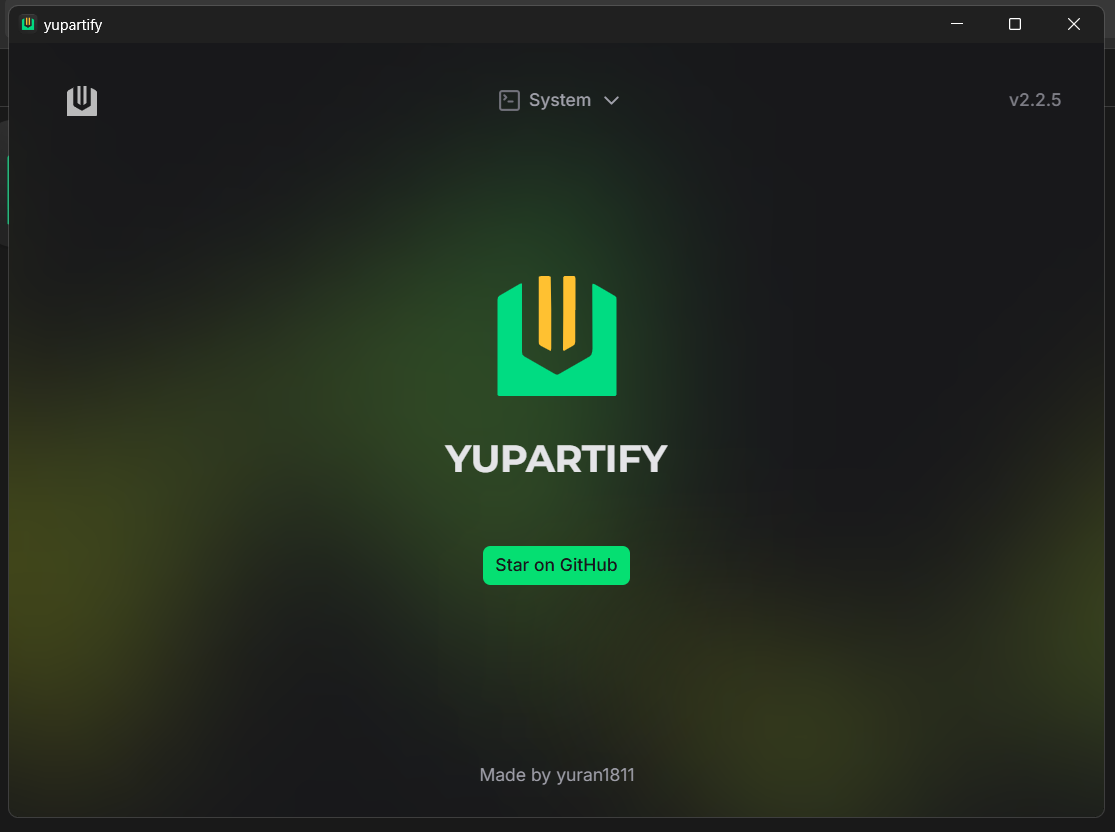
\includegraphics[width=0.9\textwidth]{../public/screenshots/home.png}
        \caption{Home page}
    \end{subfigure}
    \hfill
    \begin{subfigure}{0.47\textwidth}
        \centering
        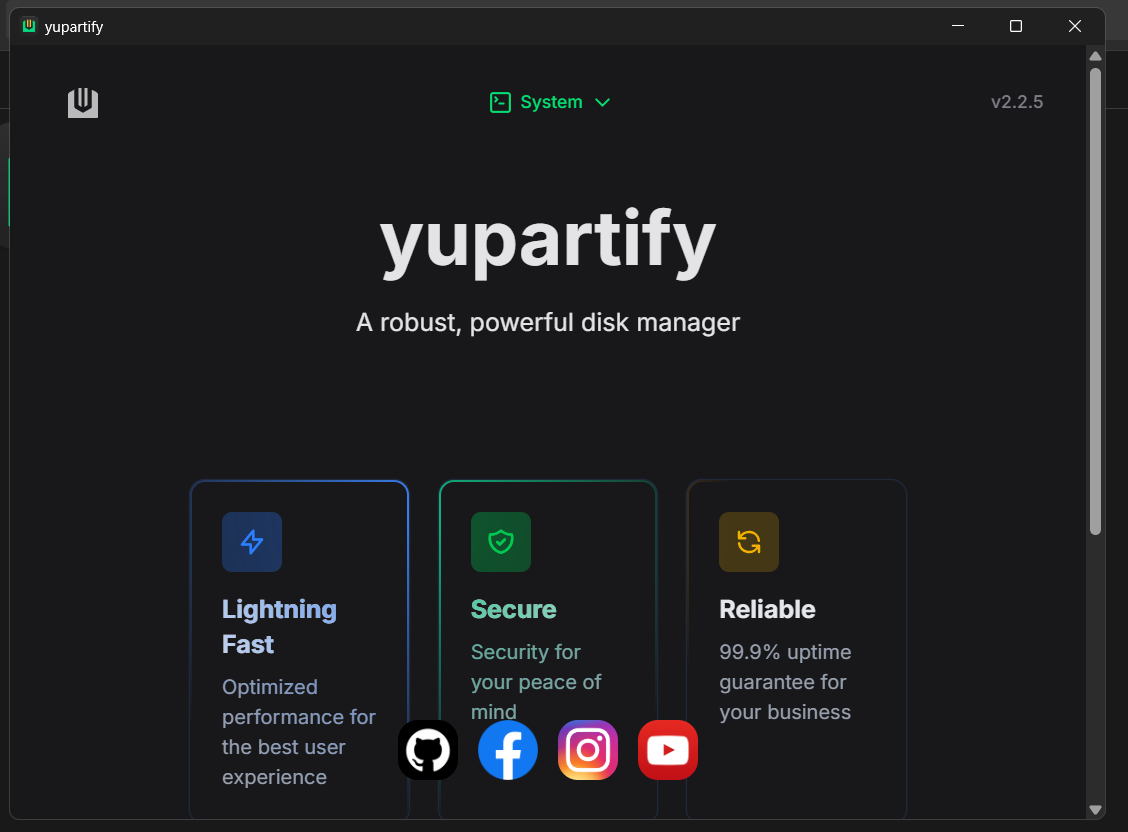
\includegraphics[width=0.9\textwidth]{../public/screenshots/about.png}
        \caption{About page}
    \end{subfigure}
    \hfill
    \begin{subfigure}{0.47\textwidth}
        \centering
        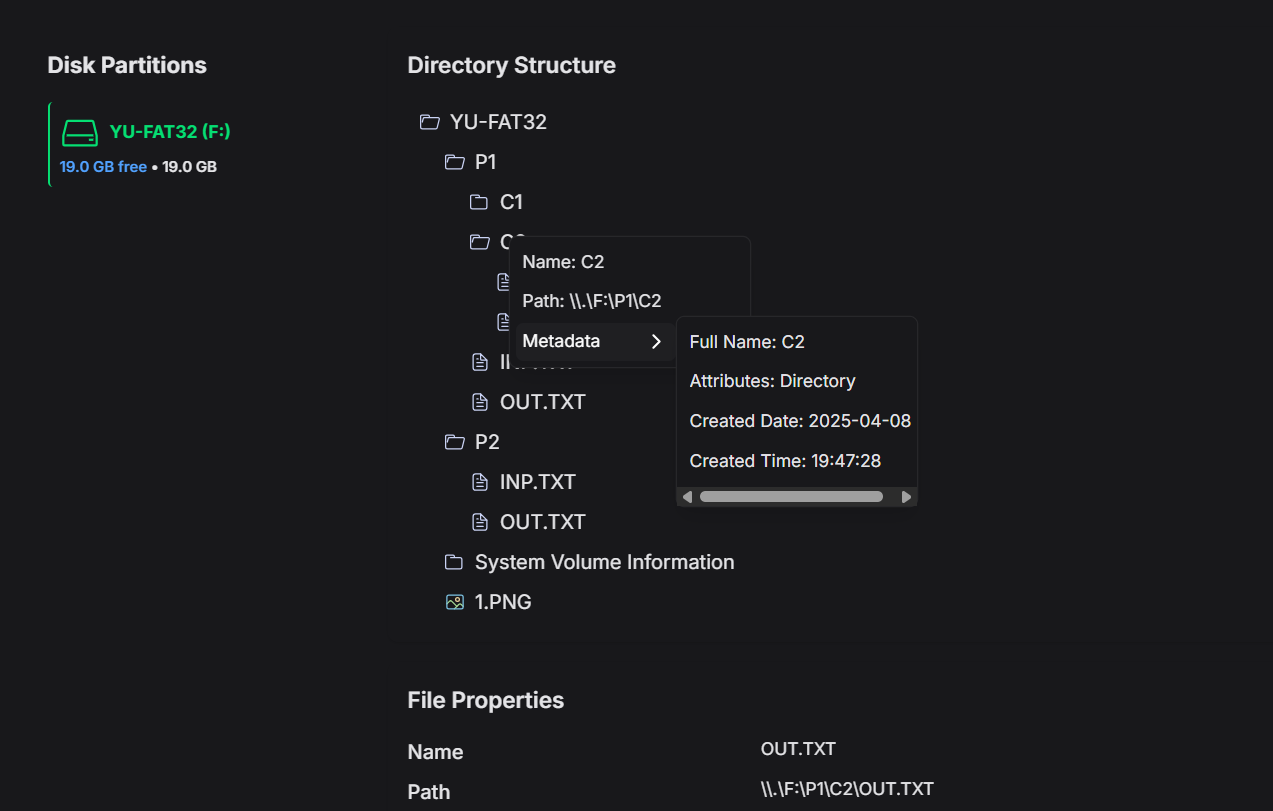
\includegraphics[width=0.9\textwidth]{../public/screenshots/dir.png}
        \caption{Display directory tree with metadata on right-click}
    \end{subfigure}
    \hfill
    \begin{subfigure}{0.47\textwidth}
        \centering
        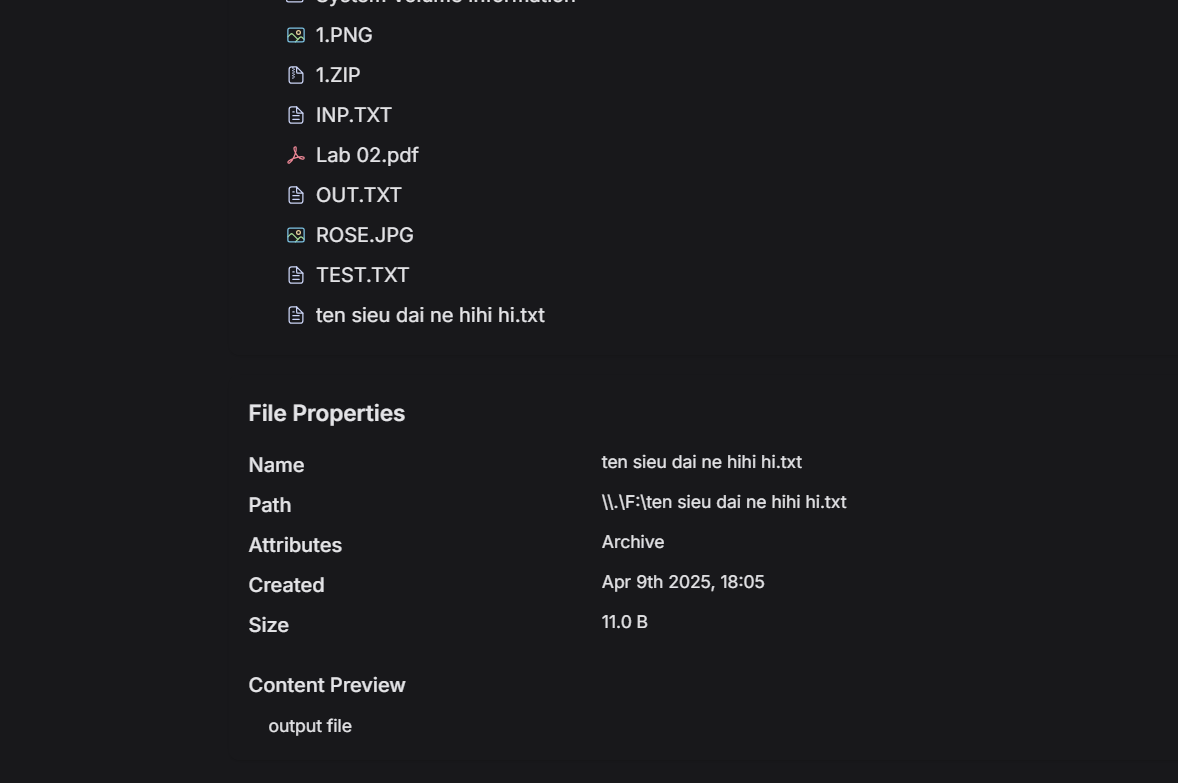
\includegraphics[width=0.9\textwidth]{../public/screenshots/file-content.png}
        \caption{Display text file}
    \end{subfigure}
    \caption{GUI App Screenshots}
\end{figure}
\begin{figure}[!ht]
    \centering
    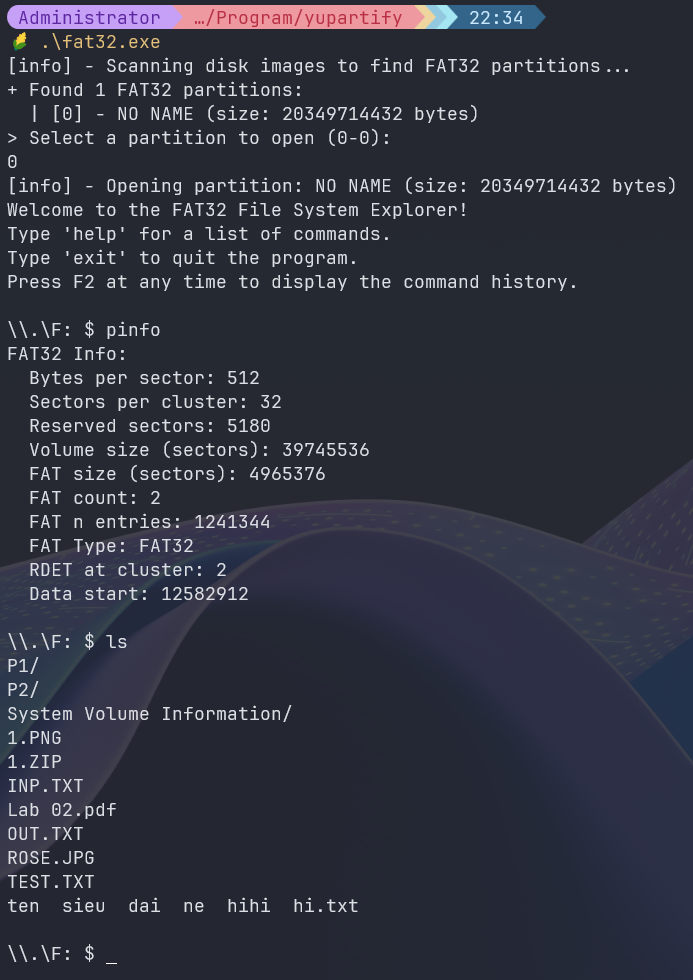
\includegraphics[width=0.9\textwidth]{../public/screenshots/cli.png}
    \caption{CLI Version}
\end{figure}

\pagebreak
\section{Project in details}
\subsection{Utility Function Implementations}
\subsubsection*{Convert numbers from little-endian bytes}
\begin{minted}{rust}
// src-tauri/src/utils/data/reader.rs
pub fn read_u16_le(bytes: &[u8]) -> u16;
pub fn read_u24_le(bytes: &[u8]) -> u32;
pub fn read_u32_le(bytes: &[u8]) -> u32;
pub fn read_u48_le(bytes: &[u8]) -> u64;
pub fn read_u64_le(bytes: &[u8]) -> u64;
\end{minted}
\subsubsection*{Other helper functions}
\begin{minted}{rust}
// src-tauri/src/utils/base.rs

// check if a file is a text file
pub fn is_text_file(path: &str) -> io::Result<bool>;

// calculate the size of a FAT32 partition based on the number of sectors used
pub fn calc_fat32_used_space(
    fats: &Vec<FATTable>,
    sectors_per_cluster: u64,
    bytes_per_sector: u64,
) -> u64;

// get attributes of a FAT32 file as a displayable string
pub fn format_attributes(attrs: u32) -> String;

// convert timestamp to a human-readable string
pub fn system_time_to_local_strings(time: SystemTime) -> (String, String);

// get the file metadata in a human-readable format
pub fn get_fat32_file_metadata(file: FATEntry) -> Result<FileMetadata, String>;
\end{minted}

\subsection{List partitions on a disk}
\subsubsection*{Read MBR}
\begin{minted}{rust}
// src-tauri/src/utils/data/reader.rs
pub fn read_mbr_disk(path: &str, partition_idx: Option<usize>) -> Result<Vec<PartitionRawInfo>> {
    if path.is_empty() || !path.starts_with(r"\\.\") {
        return Ok(vec![]);
    }

    if File::open(path).is_err() {
        return Ok(vec![]);
    }

    let mut file = File::open(path)?;
    let mut buffer = [0u8; 512];
    file.read_exact(&mut buffer)?;

    // Check boot signature
    if &buffer[0x1FE..] != [0x55, 0xAA] {
        return Err(std::io::Error::new(
            std::io::ErrorKind::InvalidData,
            "Invalid MBR boot sector",
        ));
    }

    let mut partitions = Vec::new();
    for i in 0..4 {
        // MBR disk has four partitions (16-byte entries)
        let offset = 0x1BE + i * 16;
        let entry = &buffer[offset..offset + 16];

        // ... handle partition entry
    }

    Ok(partitions)
}
\end{minted}
\subsubsection*{List FAT32 partitions}
\begin{minted}{rust}
// src-tauri/src/utils/list_partitions.rs

// list all fat32 partitions on all disks
pub fn list_fat32_paritions() -> Vec<(PartitionRawInfo, String)> {
    let mut part_list = Vec::new();

    for i in 0..32 {
        let path = format!(r"\\.\PhysicalDrive{}", i);
        match read_mbr_disk(&path, None) {
            Ok(partitions) => {
                if partitions.is_empty() && i > 0 {
                    break;
                }

                for partition in partitions.iter() {
                    if partition.raw_type.starts_with("FAT32") {
                        part_list.push((partition.clone(), path.clone()));
                    }
                }
            }
            Err(_) => {
                break;
            }
        }
    }

    part_list
}

// list all fat32 partitions on all disks with drive letter
pub fn list_fat32_paritions_by_letter() -> Vec<PartitionInfo> {
    (b'A'..=b'Z')
        .into_iter()
        .filter_map(|drive| {
            let drive_letter = format!("{}:", drive as char);
            match FAT32::open(&format!("\\\\.\\{}", drive_letter), None) {
                Ok(fat) => Some(PartitionInfo {
                    drive_letter,
                    label: fat.get_label(),
                    fs_type: fat.raw_part_info.clone().unwrap_or_default().raw_type,
                    total_size: fat.volume_size * fat.bytes_per_sector as u64,
                    free_space: fat.volume_size * fat.bytes_per_sector as u64 - fat.used_space,
                }),
                _ => None,
            }
        })
        .collect()
}
\end{minted}

\subsection{Read FAT32 file system information}
\subsubsection*{Read boot sector}
\begin{minted}{rust}
// src-tauri/src/utils/data/parser.rs
pub fn parse_boot_sector(data: &[u8]) -> FAT32BootSector {
  let bytes_per_sector = read_u16_le(&data[0xB..0xD]);
  let sectors_per_cluster = data[0xD];
  let reserved_sectors = read_u16_le(&data[0x0E..0x10]);
  let volume_size = read_u32_le(&data[0x20..0x24]);
  let fat_count = data[0x10];
  let sectors_per_fat = read_u32_le(&data[0x24..0x28]);
  let root_dir_cluster = read_u32_le(&data[0x2C..0x30]);
  let fat_type = String::from_utf8_lossy(&data[0x52..0x52 + 8])
      .trim()
      .to_string();

  let fat_size = sectors_per_fat as u64 * bytes_per_sector as u64;
  let data_start = (reserved_sectors as u64 + fat_count as u64 * sectors_per_fat as u64)
      * bytes_per_sector as u64;

  FAT32BootSector {
      bytes_per_sector,
      sectors_per_cluster,
      reserved_sectors,
      volume_size,
      fat_count,
      sectors_per_fat,
      root_dir_cluster,
      fat_size,
      fat_type,
      data_start,
  }
}
\end{minted}
\subsubsection*{Read FAT table}
\begin{minted}{rust}
// src-tauri/src/models/fat_fs.rs
impl FATTable {
    pub fn new(data: Vec<u8>) -> Self;
    pub fn is_in_bounds(&self, cluster: u32) -> bool;
    pub fn get_cluster_chain(&self, start: u32) -> Vec<u32>;
}

// src-tauri/src/utils/data/reader.rs
pub fn read_fat_table(
    file: &mut File,
    fat_count: u8,
    fat_size: u64,
    fat_start: u64,
) -> std::io::Result<Vec<FATTable>> {
    let mut raw_fats = vec![0u8; fat_size as usize];
    let mut fats = vec![];

    file.seek(SeekFrom::Start(fat_start))?;
    for _ in 0..fat_count {
        file.read_exact(&mut raw_fats)?;
        fats.push(FATTable::new(raw_fats.clone()));
    }

    Ok(fats)
}
\end{minted}
\subsubsection*{Read RDET}
\begin{minted}{rust}
// src-tauri/src/models/fat_fs.rs
#[derive(Debug, Clone)]
pub struct FATEntry {
    pub path: String,
    pub name: String,
    pub short_name: String,
    pub extension: String,
    pub attributes: FATAttributes,
    pub created: SystemTime,
    pub modified: SystemTime,
    pub accessed: SystemTime,
    pub cluster: u32,
    pub size: u32,
    pub is_deleted: bool,
    pub is_directory: bool,
}

impl FATEntry {
    pub fn is_active(&self) -> bool;
    pub fn is_valid(&self, name: &str) -> bool;
}

impl DET {
    pub fn new(data: Vec<u8>, path: &str) -> Self;
    pub fn find_entry(&self, name: &str) -> Option<FATEntry>;
    pub fn get_active_entries(&self) -> Vec<FATEntry>;
}

#[derive(Debug)]
pub struct FATClusterManager {
    pub data_start: u64,
    pub sectors_per_cluster: u64,
    pub bytes_per_sector: u64,
}

impl FATClusterManager {
    pub fn get_cluster_size(&self) -> u64;
    pub fn get_cluster_offset(&self, cluster: u64) -> u64;
    pub fn read_cluster_data(&mut self, file: &mut File, cluster: u32) -> Result<Vec<u8>>;
    pub fn read_all_cluster_data(&mut self, file: &mut File, chain: Vec<u32>) -> Result<Vec<u8>>;
}

impl FAT32 {
    pub fn open(path: &str, raw_part_info: Option<PartitionRawInfo>) -> Result<Self> {
        // ...
        let mut all_det = HashMap::new();
        all_det.insert(
            root_dir_cluster,
            DET::new(
                cluster_manager.read_all_cluster_data(
                    &mut file,
                    fats[0].get_cluster_chain(root_dir_cluster),
                )?,
                &path,
            ),
        );
        // ...
    }
}
\end{minted}
\subsubsection*{Read file content}
\begin{minted}{rust}
// src-tauri/src/models/fat_fs.rs
#[derive(Debug)]
pub struct FATClusterManager {
    pub data_start: u64,
    pub sectors_per_cluster: u64,
    pub bytes_per_sector: u64,
}

impl FATClusterManager {
    pub fn get_cluster_size(&self) -> u64 {
        self.sectors_per_cluster * self.bytes_per_sector
    }

    pub fn get_cluster_offset(&self, cluster: u64) -> u64 {
        self.data_start + (cluster - 2) * self.get_cluster_size()
    }

    pub fn read_cluster_data(&mut self, file: &mut File, cluster: u32) -> Result<Vec<u8>> {
        let mut buffer = vec![0u8; self.get_cluster_size() as usize];
        file.seek(SeekFrom::Start(self.get_cluster_offset(cluster as u64)))?;
        file.read_exact(&mut buffer)?;
        Ok(buffer)
    }

    pub fn read_all_cluster_data(&mut self, file: &mut File, chain: Vec<u32>) -> Result<Vec<u8>> {
        if chain.is_empty() {
            return Ok(vec![]);
        }

        let mut data = Vec::new();
        for cluster in chain {
            data.extend(self.read_cluster_data(file, cluster)?);
        }

        Ok(data)
    }
}

impl FAT32FileSystem for FAT32 {
  // ...
  fn read_file(&mut self, path: &str, parse_text: Option<bool>) -> Result<(Vec<u8>, String)> {
    let entry = self.fetch_file(path);
    if entry.is_err() {
        return Err(entry.unwrap_err());
    }

    let entry = entry.unwrap();
    if !entry.is_active() {
        return Ok((vec![], String::new()));
    }

    let parse_text = parse_text.unwrap_or(false);

    let chain = self.structure.fats[0].get_cluster_chain(entry.cluster);
    let mut content = Vec::with_capacity(entry.size as usize);
    for cluster in chain {
        let data = self
            .structure
            .cluster_manager
            .read_cluster_data(&mut self.file, cluster)?;

        let limit = entry.size.min(data.len() as u32) as usize;
        content.extend_from_slice(&data[0..limit]);
    }

    let parsed_content = parse_file_content(&content);

    Ok((
        content,
        if parse_text {
            parsed_content
        } else {
            String::new()
        },
    ))
  }
  // ...
}
\end{minted}

\subsection{Use with GUI}
\subsubsection*{Read directory tree}
\begin{minted}{rust}
// src-tauri/models/fat_fs.rs
pub trait FAT32FileSystem: FileSystem {
    fn cd(&mut self, path: &str) -> Result<()>;

    fn list_rdir(&mut self) -> Result<Vec<FATEntry>>;
    fn list_dir(&mut self, path: &str) -> Result<Vec<FATEntry>>;

    fn fetch_file(&mut self, path: &str) -> Result<FATEntry>;
    fn fetch_metadata(&mut self, path: &str) -> Result<(FileMetadata, Option<FATEntry>)>;

    fn read_file(&mut self, path: &str, parse_text: Option<bool>) -> Result<(Vec<u8>, String)>;

    fn read_immediate_children(&mut self, path: &str) -> Result<DirectoryNode>;
    fn build_shallow_node(&mut self, path: &str) -> Result<DirectoryNode>;
}


// src-tauri/src/lib.rs
#[tauri::command]
fn get_children(path: String) -> Result<DirectoryNode, String> {
    let cur_drive = get_store_value("working_drive");
    if cur_drive.is_none() {
        return Err("No current drive found in store".to_string());
    }

    let cur_drive = cur_drive.unwrap();
    let part = format!("\\\\.\\{}", cur_drive["label"].as_str().unwrap());
    match FAT32::open(&part, None) {
        Ok(mut f) => match f.read_immediate_children(&path) {
            Ok(children) => Ok(children),
            Err(_) => Err("Error reading children".to_string()),
        },
        Err(_) => Err("Error opening FAT32".to_string()),
    }
}
\end{minted}
\subsubsection*{Read file content}
\begin{minted}{rust}
// src-tauri/src/lib.rs
#[tauri::command]
fn read_text_file(path: String) -> Result<String, String> {
    let cur_drive = get_store_value("working_drive");
    if cur_drive.is_none() {
        return Err("No current drive found in store".to_string());
    }

    let cur_drive = cur_drive.unwrap();
    let part = format!("\\\\.\\{}", cur_drive["label"].as_str().unwrap());
    match FAT32::open(&part, None) {
        Ok(mut f) => match f.read_file(&path, Some(true)) {
            Ok((_, content)) => Ok(content),
            Err(_) => Err("Error reading file".to_string()),
        },
        Err(_) => Err("Error opening FAT32".to_string()),
    }
}
\end{minted}

% References
\pagebreak
\section{References}
\begin{enumerate}
    \item \href{https://github.com/NicolaSpadari/nuxtor}{nuxtor}: Tauri + Nuxt starter template for the GUI\@.
    \item \href{https://www.deepseek.com/}{DeepSeek}, \href{https://chatgpt.com/}{ChatGPT}: AI Agents help to implement the FAT32 file system and write helper functions.
    \item \href{https://github.com/PSDat123/FAT32-and-NTFS-explorer/blob/master/FAT32.py}{FAT32 explorer}: Take inspiration from this Python implementation ver of FAT32 file system.
\end{enumerate}
\end{document}
